\section{\centering Untyped \lCalc}
In order to get acquainted with the \lcalc, let us develop a simple example to familiarize ourselves before we begin with a more formal approach to this discipline. Consider the function $f(x) = x + 1$, the most straightforward way to express this using \lcalc \ would be $(\la x . x + 1 )$, where the lambda denotes that $x$ is being captured and used as a parameter to perform some computation\footnote{this is an example, $(\la x . x + 1 )$ is not a valid lambda term, see Definition \ref{def:lambda-terms-2}.}. Evaluating $f(2)$ using this newly created lambda term would look like this: $(\la x . x + 1)(2) \curly (2 + 1) \curly 3$. This process of reducing a $\la$-expression is referred to as \bred, it will be covered formally later in the chapter.

\begin{definition} The set of all lambda terms \( \La \) is defined inductively as follows:
  \label{def:lambda-terms-1}
  \begin{itemize}
  \item (Variable) If \( x \in \Vset \), then \( x \in \La \).  
  \item (Abstraction) If \( x \in \Vset \) and \( M \in \La \), then \( (\la x. M) \in \La \).
  \item (Application) If \( M, N \in \La \), then \((M N) \in \La \).
  \end{itemize}
  Where $\Vset = \{x, y, z, ... \}$ represents a countably infinite set of variable names.
\end{definition}
  
The key takeaway of this definition is that abstraction and application together, when combined with \bred, enable computation—thus encapsulating the meaning of function in a way that is abstract yet useful.

Since we are dealing with a formal language, it is in our benefit to introduce a few other objects with the aim of defining a grammar to generate the set $\La$:
\begin{itemize}
\item An alphabet \( \Sigma = \{ \la, ., (, ), \ldots \} \), is a finite set of symbols
\item A string is a finite sequence of elements from \( \Sigma \), the empty string is denoted by \( \varepsilon \)
\item \( \Sigma^* \) denotes the set of all finite strings over \( \Sigma \), \( \varepsilon \in \Sigma^* \)
\item A language \( L \) over an alphabet \( \Sigma \) is a subset of \( \Sigma^* \)
\end{itemize}
Our aim now, to generate the set $\La$,  to do this, we will make use of a grammar. When dealing with grammars that define programming languages i.e. context-free grammars, Backus-Naur Form, BNF for short is the way to go:
\begin{itemize}
\item Nonterminals are enclosed in angle brackets (e.g. \texttt{<expr>})
\item Terminals are written literally (e.g. \texttt{"$\lambda$"}, \texttt{"."}, $x$)
\item Productions define how nonterminals expand, written as \texttt{::=}
\item The vertical bar \texttt{|} denotes available expansions
\end{itemize}
Thus, the language for natural numbers in decimal notation is represented using:
\begin{align*}
  \texttt{<digit>} &\;\texttt{::=}\; \texttt{"0"} \;\texttt{|}\; \texttt{"1"} \;\texttt{|}\; \texttt{"2"} \;\texttt{|}\; \texttt{"3"} \;\texttt{|}\; \texttt{"4"} \;\texttt{|}\; \texttt{"5"} \;\texttt{|}\; \texttt{"6"} \;\texttt{|}\; \texttt{"7"} \;\texttt{|}\; \texttt{"8"} \;\texttt{|}\; \texttt{"9"} \\
  \texttt{<number>} &\;\texttt{::=}\; \texttt{<digit>} \;|\; \texttt{<digit>} \ \texttt{<number>}
\end{align*}
\begin{definition} Taking advantage of BNF notation, an alternative definition for $\La$ would be:
  \label{def:lambda-terms-2}
  \begin{align*}
    \texttt{<term>} &\;\texttt{::=}\; \texttt{<variable>} \\
                    &\;\texttt{|}\; \texttt{"$\la$"}\ \texttt{<variable>}\ \texttt{"."}\ \texttt{<term>} \\
                    &\;\texttt{|}\; \texttt{"("}\ \texttt{<term>}\ \texttt{<term>}\ \texttt{")"} \\
    \texttt{<variable>} &\;\texttt{::}\in \Vset
  \end{align*}
  where \( \Sigma = \{ \la, ., (, )\} \cup \Vset \) and \( \La \subset \Sigma^* \). Through use of inductive types types\footnote{Inductive Data Types are inductively defined types built from sums (either this or that) of products (this and that). They let you define structured data with multiple forms and support safe, exhaustive pattern matching.}, this grammar can be implemented in Lean4:

\end{definition}
\begin{remark}
  From the definition above we extract that \( \lambda x . x + 1 \notin \La \), given this circumstance, the need to find an accurate representation for numbers within this definition arises. See Definition \ref{def:church-naturals}
\end{remark}
\begin{example} \label{ex:lambda-terms} Some examples of valid $\la$ terms generated using the grammar in \ref{def:lambda-terms-2}:
  \( y \),
  \( (\la x. (x x)) \),
  \( (\la x. (\la y. x)) \),
  \( (((\la x. (x y)) (\la y. y)) z) \).
  The Lean4 counterpart for the second term is:
\end{example}
As a convention to avoid notational cluttering, the outermost parenthesis can be omitted e.g. $ ( \la x.x ) $ can be read as $ \la x.x $. Also, application is left-associative  and binds tighter than abstraction, so $M N P$ is parsed as $(M N) P$ and $\la x . M N$ means $\la x . (M N)$, not $(\la x . M) N$. Likewise, abstraction is right-associative e.g. $\la x . \la y . M$ is $\la x . (\la y . M)$ and binds more weakly than application. All these are just to keep notation straight-forward, the formal definition does not leave precedence under-specified thanks to parenthesis. Those interested in the implementation need not worry, as Lean4 enforces an explicit order on constructors.
\subsection{\centering Equivalence of terms}
Having defined the language of the \lcalc, we move on to the mechanics of computation. To this end, several equivalences among terms will be defined, namely \aequiv, \bequiv, and \etaequiv
. Every lambda term is made up of other smaller lambda terms, so it is only natural to define the set that contains all subterms of a given term:
\begin{definition} Given $T \in \La$, $\functionfont{Sub} : \La \to \mathcal{P}(\Vset)$ maps a term to the set of it's subterms.
  \begin{align*}
    &\Sub x = \{x\} \\
    &\Sub {MN} = \Sub M  \cup \Sub N \cup \{MN\} \\
    &\Sub {\la x . M} = \Sub M  \cup \{\la x. M\}
  \end{align*}
  Where $x \in \Vset$ and $M, N \in \La $.

\end{definition}
\begin{remark}
  Let \( \preceq \) be the subterm relation on \lterms, defined by
  \[
    M \preceq N \iff M \in \Sub{ N }
  \]
  \( \preceq \) is a partial order relation. This statement is follows intuitively from the definition, it can be proven using induction on the derivation tree.
\end{remark}
\begin{definition} A term $ S \in \Sub M, \ M \in \La$ is said to be proper if $S \neq M$. $\Sub{M} \setminus \{M\}$ would be the set of proper subterms.
\end{definition}
\begin{definition} Let \( M = \lambda x. N \) be a \lterm:
  \begin{itemize}
  \item The variable \( x \) is the binding variable of the abstraction \( \lambda x. N \).
  \item An occurrence of a variable \( x \) in \( M \) is bound if \( x \in \Sub { \lambda x. N } \).
  \item Free variables are those that are not bound.
  \end{itemize}
\end{definition}
\begin{example}
  Take $ M \equiv \la x . \, x \, y $, in this example, the $x$ in $\la x. $ is binding, $y$ is free, and $x$ is bound. This means that $y$ is used literally, and that $x$, as denoted by $\la x.$ is abstracted and thus subject to being replaced within the context of said abtraction. A subexample might make this explicit: $ (\la x . \, x \, y) \, M \curly M \, y $. The $y$ remained while the $x$ was used as a placeholder for $M$.
\end{example}
\begin{remark}
  This taxonomy is key to understanding concepts such as \aequiv \ intuitively.
\end{remark}
The set of Free Variables $\functionfont{FV}$, those that will not get replaced during the process of reduction, is computed using:
\begin{definition} Given $T \in \La $, $\functionfont{FV} : \La \to \mathcal{P}(\Vset) $ outputs the set of free variables for $T$:
  \begin{align*}
    & \FV x = \{x\}\\
    & \FV {MN} = \FV M \cup \FV N \\
    & \FV {\lambda x . M} = \FV M \setminus \{x\}
  \end{align*}
  Where $ x \in \Vset $ and $ M, N \in \La $, and $\mathcal{P}$ denotes the power set.

\end{definition}
\begin{example} Computing the free variables of $\lambda x . \lambda y . y x z$. The term well-formed, so we proceed:
  \begin{align*}
    \FV {\lambda x . \lambda y . y x z} &= \FV {\lambda y . yxz} \setminus \{x\} \\
                                        &= \FV {yxz} \setminus \{x, y\} \\
                                        &= \{x, y, z\} \setminus \{x, y\} \\
                                        &= \{z\}
  \end{align*}
  Of course, $z$ is the only free variable in the expression as it is the only variable that is not captured by some $\la$-abstraction.
\end{example}
\begin{definition}
  A term $M \in \La$ is closed if and only if $\FV M = \emptyset$, closed lambda terms are often referred to as combinators. $\La^0$ is the set of all closed lambda terms.
\end{definition}
\begin{note} They are called combinators since having no free variables means that all variables are bound, and thus, a closed term just combines bound variables.
\end{note}

We approach the definition for \aequiv \, to this end we have to introduce what it means to substitute a variable.

\begin{definition}Capture-Avoiding Substitution Rules
  Let \( M, N \in \La \) and \( x, y, z \in \Vset \). The substitution \( M[x := N] \) is defined inductively as:
  \[
    \begin{aligned}
      x[x := N]                       & = N \\
      y[x := N]                       & = y && y \neq x \\
      (M_1\, M_2)[x := N]             & = (M_1[x := N])\,(M_2[x := N]) \\
      (\lambda x. M)[x := N]          & = \lambda x. M \\
      (\lambda y. M)[x := N]          & = \lambda y. (M[x := N]) && y \neq x, y \notin \FV { N } \\
      (\lambda y. M)[x := N]          & = \lambda z. (M[y := z][x := N]) && y \neq x, y \in \FV { N }
    \end{aligned}
  \]
  where \( z \notin \FV { M } \cup \FV { N } \).
\end{definition}
Hopefully the meaning of the first three rules is clear, they ancapsulate renaming in the context of variables and applications. The subsequent rules are about abstractions, rule four states that renaming a binding variable has no effect, renaming only modifies a term whenever the renamed variable is different from the binding variable. Rule five is the general case, that is, when the substitution just moves in together with the abstracted term. Then there is the last case, when the binding variable is a bound occurrence in the term we are substituting, which poses a problem, to see why, let us work through an example:
\begin{example} If by mistake we substitute $x$ by \( (\la w . \, w \, y) \) in \( (\la y . \, y \, x ) \) using rule five, we get:
  \[
    (\la y . \, y x) [x := (\la w . \, w \, y)] = (\la y . \, y \, (\la w. \, w \, y))
  \]
  This is problematic since the free variable $y$ became bound after the rename. Free and bound variables should mantain their freedom or their boundedness after the rename, hence the need for rule 6, where we rename the binding variable to avoid the name clash:
  \[
    (\la y . \, y x) [x := (\la w . \, w \, y)] = (\la z . \, z \, (\la w. \, w \, y))
  \]
  The purpuse of the binding variable is to serve as a placeholder, therefore renaming does not affect the integrity of the expression, the variable gets replaced anyway when we perform a reduction.
\end{example}
In the previous example a bound variable is renamed to avoid a naming collision and avoid binding a previously free variable, \aequiv \ is the generalization of this technique, it defines equivalence up to renaming of binding variables.
\begin{definition} Two lambda terms \( M, N \in \La \) are \aequivlt, written \( M =_\alpha N \), if they are structurally identical except for the names of bound variables.
  Formally:
  \[
    \begin{array}{@{}l@{\quad}l@{}}
      \inferrule*[right=\textsc{Alpha}]
      { }
      { \lam{x}{L} =_\alpha \la y . \, L \subst{x}{y} }
      &
        \inferrule*[right=\textsc{Abs}]
        { L =_\alpha L' }
        { \lam{x}{L} =_\alpha \lam{x}{L'} } \\[2ex]
      \inferrule*[right=\textsc{AppL}]
      { L_1 =_\alpha L_1' }
      { L_1\,L_2 =_\alpha L_1'\,L_2 }
      &
        \inferrule*[right=\textsc{AppR}]
        { L_2 =_\alpha L_2' }
        { L_1\,L_2 =_\alpha L_1\,L_2' }
    \end{array}
  \]
  $\alpha$-equivalence is an equivalence relation:
  \[
    \begin{aligned}
      &(Reflexivity) \quad && M =_\alpha M \\
      &(Symetry) \quad && M =_\alpha N \Rightarrow N =_\alpha M \\ 
      &(Transitivity) \quad && M =_\alpha N \text{ and } N =_\alpha P \Rightarrow M =_\alpha P
    \end{aligned}
  \]
\end{definition}
\begin{example} A simple equivalence class and two samples of not $\alpha$-equivalent \ pairs.
  \[
    \la x.\la y. \, y =_\alpha \la a.\la b. \, b =_\alpha \la z.\la x. \, x
  \]
  \[
    \la x. \la y. \, x \not=_\alpha \la x. \la y. \, y \quad \la x. \, x \, y \not=_\alpha \la x. \, x \, z 
  \]
  Remember terms are $\alpha$-equivalent \ only when bounded names are properly substituted.
\end{example}
\begin{remark}
  \aequiv \ comes naturally once substitution is defined, since the names of bound variables are just placeholders whose only purpuse is to get replaced.
\end{remark}
Naming variables can be a nightmare, which is why there exists a way of methodically assigning numbers to variables in a way that eliminates the need for \aequiv. These naming system works by using numeric indices that indicate how many binders away a variable’s binder is. These indices are called De Bruijn indeces.
\[
  \la x.\, x \Rightarrow \la.\, 0 \quad \la x. \la y.\, x \Rightarrow \la. \la.\, 1 \quad \la x. \la y.\, y \Rightarrow \la. \la. \, 0\,
\]
It turns out we are better at naming variables than at working with numbers, which is why we will stick to symbols and leave De Bruijn indices to computers. Programs like automated theorem provers do use this naming strategy to simplify their work.

\begin{definition} Single-step $\beta$-reduction $\step$ is defined using the following inference rules:
\[
\begin{array}{@{}l@{\quad}l@{}}
  \inferrule*[right=\textsc{Beta}]
    { }
    { (\lam{x}{M})\,N \step M\subst{x}{N} }
  &
  \inferrule*[right=\textsc{Abs}]
    { M \step M' }
    { \lam{x}{M} \step \lam{x}{M'} } \\[2ex]
  \inferrule*[right=\textsc{AppL}]
    { M_1 \step M_1' }
    { M_1\,M_2 \step M_1'\,M_2 }
  &
  \inferrule*[right=\textsc{AppR}]
    { M_2 \step M_2' }
    { M_1\,M_2 \step M_1\,M_2' }
\end{array}
\]
where \( M, N \in \La \). For those not familiar with inference rules, here is an alternative definition where \( L \in \La \)
\begin{itemize}
\item \( (\lam{x}{M})\,N \step M\subst{x}{N} \)
\item If $M \step N$, then: \( M\,L \step N\,L; L\,M \step L\,N; \lam{x}{M} \step \lam{x}{N} \)
\end{itemize}
\end{definition} 
Single \bred s can be applied succesively, which induces the following definition
\begin{definition} Zero or more step \bred, the reflexive transitive closure of \bred. We write $M \step^* N$ if and only if there exists a sequence of one-step $\beta$-reductions starting from $M$ and ending at $N$.\footnote{The convention in the literature is to use $\rightarrow_\beta$ for \bred s $\twoheadrightarrow_\beta$ for multi-step \bred s. I prefer to use $\curly$ and $\curly^n$ since this allows me to use the superscript to note the number of steps in the process \bred \ e.g. $ (\la f. \la x . \, x) \, M \, N \curly^2 $ N. Instead of $\curly^n$ I use $\curly^*$ whenever the number of steps is undefined.}
  \label{def:zero-more-bred}
  \[
    M \equiv M_0 \step M_1 \step M_2 \step \cdots \step M_{n-1} \step M_n \equiv N
  \]
  That is, there exists an integer $n \geq 0$ and a sequence of terms $M_0, M_1, \dots, M_n$ such that: $ M_0 \equiv M $ and $ M_n \equiv N $ for all $ i $ with $ 0 \leq i < n $, we have $ M_i \step M_{i+1} $.
\end{definition}
The process of succesively $\beta$-reducing a term leads raises the question of whether all terms can be reduced indefinitly. We know the answer to this, since for instance, variables in $\Vset$ cannot be reduced. The subsequent question is then, Do all all terms have some kind of normal form that cannot be reduced further? This is answered in Section \myref{sec:recursion-fixed-points}.
\begin{definition} \bequiv \ relation, equivalence of \lterms \ through \bred s.
  \[
    M =_\beta N \iff M \step^* N \lor N \step^* M
  \]
 Using definition \ref{def:zero-more-bred}:
  \[
    M =_\beta N \iff
    \begin{cases}
      \exists M_0, \dots, M_n \text{ s.t. } M \equiv M_0 \curly M_1 \curly \cdots \curly M_n \equiv N \\
      \exists N_0, \dots, N_n \text{ s.t. } N \equiv N_0 \curly N_1 \curly \cdots \curly N_n \equiv M
    \end{cases}
  \]
\end{definition}
\begin{remark}
  In the context of equivalence of programs, \bequiv \ can be understood as means for intensional equivalece, the kind of equivalence that requires programs to be equivalent in a step-by-step fashion.
\end{remark}
We now explore a key aspect of the \lcalc, in the jargon referred to as first-class citizenship, or high-order, a property of terms that restrains them from being exclusively classified as either function or argument. The example below sheds some light on the matter:
\begin{example} High Order by example. Let us $\beta$-reduce the \lterm \ $ A \, B \, C $ and inspect the consequences:
  \label{ex:high-order-by-example}
\begin{align*}
  \overbrace { (\lambda f . \lambda y . f f y) }^{A} \overbrace{ (\lambda x . x + 1) }^{B} \overbrace{(2)}^{C}
  &\curly (\lambda y .(\lambda x . x + 1) (\lambda x . x + 1)y)(2) \\
  &\curly (\lambda x . x + 1)(\lambda x . x + 1)(2) \\
  &\curly^* (\lambda x . x + 1) (3) \\
  &\curly^* (4)
\end{align*}
Taking a closer look, $A$, applies $f$ twice to $x$, as a consequence, $B$ is being applied twice to $C$. And so, very easily, we have implemented the $ x + 2 $ function via a sequential application of $x + 1$ to $C$.
\end{example}
\begin{remark}
  As seen above, we can pass what we understand as conventional functions as arguments since they are treated alike.  One can intuitively apreciate the computational expresivenes this brings with it, and how this syntactic-semantic homogeneity sets the \lcalc \ apart from the classical set-theoretic approach to functions.
\end{remark}

\begin{theorem} The Church-Rosser Property states that $\forall M, N_1, N_2 \in \La$:
  \[
    M \curly^* N_1 \quad \text{and} \quad M \curly^* N_2 \quad \Rightarrow \quad \exists N_3 \, \mid \, N_1 \curly^* N_3 \,\wedge\, N_2 \curly^* N_3
  \]
  If a lambda term $M$ has a normal form, then every reduction sequence starting from $M$ eventually reduces to that same normal form, up to alpha-equivalence. The diagram below is the reason this theorem is often referred to as the diamond property.
\begin{center}
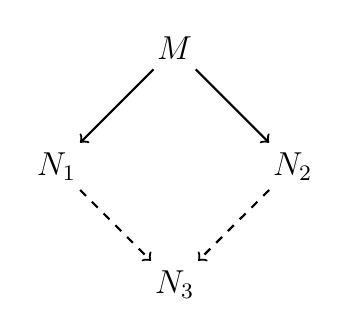
\begin{tikzpicture}[node distance=2.0cm, every node/.style={font=\large}]
  \node (t) at (0,0) {$M$};
  \node (t1) at (-1.5,-1.5) {$N_1$};
  \node (t2) at (1.5,-1.5) {$N_2$};
  \node (t3) at (0,-3) {$N_3$};
  \draw[->, thick] (t) -- (t1) node[midway, above left] {}; %{$\curly^*$};
  \draw[->, thick] (t) -- (t2) node[midway, above right] {}; %{$\curly^*$};
  \draw[->, dashed, thick] (t1) -- (t3) node[midway, below left] {}; %{$\curly^*$};
  \draw[->, dashed, thick] (t2) -- (t3) node[midway, below right] {}; %{$\curly^*$};
\end{tikzpicture}
\end{center}
The proof to this theorem is a quite lengthy, we would be miss the point
of this document if we were to introduce it [ChurchRosser].
\end{theorem}
\begin{corollary} Normalization: If a $\lambda$-term $M$ reduces to two normal forms $N_1$ and $N_2$, then they are alpha-equivalent:
\[
M \to_\beta^* N_1 \ \ \text{and} \ \ M \to_\beta^* N_2 \ \ \text{and $N_1$, $N_2$ are normal} \ \ \Rightarrow \ \ N_1 =_\alpha N_2
\]
\end{corollary}
The last and indeed the least important notion of equivalence:
\begin{definition} Two lambda terms \( M \) and \( N \) are said to be $\eta$-equivalent, written \( M =_\eta N \), if:
  \[
\begin{array}{@{}l@{\quad}l@{}}
  \inferrule*[right=\textsc{Eta}]
  { x \notin \FV M }
  { (\lam{x}{M}) =_\eta M   }
  &
  \inferrule*[right=\textsc{Abs}]
    { M =_\eta M' }
    { \lam{x}{M} =_\eta \lam{x}{M'} } \\[2ex]
  \inferrule*[right=\textsc{AppL}]
    { M_1 =_\eta M_1' }
    { M_1\,M_2 =_\eta M_1'\,M_2 }
  &
  \inferrule*[right=\textsc{AppR}]
    { M_2 =_\eta M_2' }
    { M_1\,M_2 =_\eta M_1\,M_2' }
\end{array}
\]

The abstraction \( \lambda x.\, (M\;x) \) performs the same operation as \( M \), so if \( x \) is not used freely within \( M \), the abstraction is redundant. This is shown in \textsc{Eta}, the rest of the inference rules propagate this equivalence onto the whole term. Put into programming the idea becomes trivial: \orange{pseudo code example. given f of type , def g (n) := f n is equivalent to just calling g.}

\end{definition}
$\eta$-equivalence represents weak extensionality, since it does not encode observational equivalence. Two terms are observationally equivalent if they cannot be distinguished by any context that can be papplied to them.
